In this work we define the chronological order assuming any possible combination of event assortment. We assume there is no golden order for any set of events, when we hypothesise in terms of feasible outcomes, in which we rely on the existence of more or less favourable cases.
\\
\subsection{Chronological order of mutation impact disease evolution}

%Example of order irrelevance
An unordered model under system's biological dynamics, i.e. a system not bound to temporal order, is our main assumption for gene interaction. On the other hand, we hypothesise chronological order existence within this freedom.

Sufficient backing studies to confirm order is in (or has) control of/over the full dynamics of the system are not available, hence a order-driven hypothesis cannot be proven. However, some of the above mentioned projects have accurately identified the effects chronological order has in case evolution, which manifest the scenario is plausible. 

This fact serves as motivation to study conditions where general conclusions made up til now are not sufficient, and consider heterogeneity as a order-related issue.
\\

%Hybrid
Furthermore, an hybrid system managing the dynamics of the clonal population can even find the balance among both proposals. E.g. in \cite{Ascolani2019ModelingMatter} we have observed order in CD47 and CD44 mutations is not relevant. Assuming an ordered model, in which a set of events are known to be sequential, this scenario might be feasible as well because their chronological order can be swapped without altering it. In a non-ordered model, the reason is trivial. Interestingly, the hybrid model (loosely ordered), accepts sequential order at some points, and gets more relaxed with synonymous ordered events. A strict total-order driven occurrence of events is not probable.
\\

To simplify this estimation, we also assume no other interaction interfere with the model, albeit the scenario is far from probable as cancer complexity cannot be studied leaving interaction out. Clones build an established microenvironment in which, although might be lacking vital functions such as specific signal detection from external sources, communication amongst the members is still possible \cite{Chiodoni2019Correction10.1186/s13046-019-1122-2}. The subclonal population is still present in the organism where the cancer developing, therefore this interaction must also be taken into consideration.
\\
%Event assorting evolution (and eventual branching) also opens up the %discussion between linear and parallel metastasis progression models %\cite{Turajlic2016MetastasisProcess}.

Based on the cases above, we can then confirm event chronological order is relevant for prognosis, yet it entirely depends on the condition we are facing, beside environment. The weight of its impact remains bound to environment and issues we discuss later in this section. Given most of the studies have examined conditions affecting a large portion of the population, we can only trust additional expertise will be gathered in the future.

%Unleashing the applications
Chronological order establishment is the main requirement to unleash the next stage  of oncologic studies which eventually leads to clinical application. Constituting this assortment then becomes the main challenge for the oncogenic field \cite{Gerstung2011TheTumorigenesis} based on the fact that clones can show vast clinical and histological differences, even when common (overlapping) mutations are present. However, as shown in the \cite{Fearon1990ATumorigenesis} example, an order preference is reasonable to consider, but it does not set a strict rule. Events such as sudden point mutations can produce an alteration event which was expected late in the progression rather than driven due to a cascade result. E.g. in \cite{Ascolani2019ModelingMatter} EPCAM is the first mutation to happen, and MET is the last. MET can mutate in early stages provoked by other events, not the EPCAM event triggering it, then their order, at clinical analysis, has been inverted. Yet, generally, EPCAM before MET is \emph{preferred}, probably due to the low probability of conditions which altered MET unusually.
\\

\subsubsection{General heterogeneity}
Clonal diversity is caused by divergent events evolution within the neighbourhood, which in turn happens due to the microenvironment conditioning. This unleashes a myriad of scenarios at sample analysis, from cases where equal mutations have accumulated but they were acquired in different order, to populations holding the same progression but in which cell cycles differ, among others. Both presented perspectives often fail at presenting predictive biomarkers, and generally result in different subtypes within a condition. 

\cite{Herbet2012AcquisitionPhenotypes} shows a clear example of this onset in the myeloprolifertive neoplasm condition, in which discerning between two clearly differentiated progressions (genetically and phenotipically) can be done smoother than in others.
\\

Although the degree of discernment in other conditions remains largely unknown, large heterogeneity within the clonal population could be analysed via phylogenetic trees analysis, and present a starting scenario from which order can be retrieved.

Based on the studies above, we know a full phylogenetic scenario displaying is challenging to retrieve, since the environment might contain a conglomerate of multiple divergent-evolved clones. Even so, many studies attempt to display the divergent scenario as accurately as possible  via phylogenetics \cite{Beerenwinkel2005Mtreemix:Trees} \cite{Rahnenfuhrer2005EstimatingScores}, or networks \cite{Hjelm2006NewOncogenesis} \cite{Gerstung2011TheTumorigenesis}. Mainly they would aim at establishing most of the events in a timeline that can be used as support for tracing. Patient stratification becomes then a temporal issue \footnote{Defining a chronological system in which events are not strictly linear results in a branched scheme. Automata theory and Computational Tree Logic (CTL) model support this approach and offer good visualisations of the scenarios.}, still based on snapshots, although having a broader view on prognosis.

It would also be a step forward in terms of heterogeneous clones eradication, which are the main issue when it comes to patient's relapse.

\subsubsection{External interactions consideration}
Meta knowledge can be added to the study to aid chronological organisation as reinforcement for ambiguous cases, given the effects and evolution of mutations are known. E.g, based on TNM staging system, clone starting node point evasion and tissue invasion is expected —although not limited to \cite{Turajlic2016MetastasisProcess}— in stage 4, therefore, effective driver mutations are expected later in the phylogenetic-tree-like model. Having a shallow prediction of an event belonging is highly indicative in terms of guiding the research.
\\

Based on an evolutionary argument, there is also a \emph{weighting} effect on each mutation. Some driver mutations can be more harmful than others when it comes to consequences regarding behaviour down the line. E.g. cell's apoptosis control system disruption generally initiates cancer. In terms of fitness, the more the progeny grows, the higher is the probability of alterations acquisition which enter the game of survival\cite{Gerstung2011TheTumorigenesis}. Therefore, alterations driving apoptosis should be tagged as more risky in terms of prognosis. Radical-stage inducing events such as apoptosis, cooperation loss, proliferation, metastasis, etc. are highly relevant for the cause.
\\

\subsubsection{Clinical meaning and application}
Assuming historical order establishment, case classification, patient stratification and evolution prediction can entirely rely on stage’ history traceback analysis. Chronological ordering of events offers a small grained display of the scenario, then tracing would be based on evolution and not on a single (current) snapshot. We must keep in mind then, a parallel progression model \cite{Turajlic2016MetastasisProcess} is also feasible, considering the intricate dynamics of pathways interaction, in which one element can arouse the misbehaviour of many.
\\

Pinpointing the exact stage of a cancer evolution having knowledge of past events leaves us with a highly sensitive model that helps us act on the most effective spot to break more lethal consequences.

Given the full spectrum of possibilities in which events can occur due to pure systems dynamics, the deductions and proposed lines of research can seem strict. However, they are not meant to solve the entire organisation by setting an order of mutations for each condition, but to offer some more insight about which are the lines that regulate cancer prognosis.

% -------------
% Pathways
\subsection{Pathways disruptions}
%Grain
The grain of the methodology is related to the defects it might encounter. Previously, gene-based approaches looking for a rule of chronological order offers a precise point of action if the discovery is made. Strictness of such models shall be controlled by hyperparameters which tolerate divergence, e.g. interchangeable orders, irrelevant items (noise) and so on.

%Drawbacks
This drawback seems to be solved on pathway-based due to its system-like behaviour: if any member of the pathway gene set is altered, this affects the full network which has any interaction with it, which eventually triggers a cascade effect, disrupting all systems directly related to them. Therefore, looking at the problem from a \emph{wider} view, whose focus now is on setting order among pathways instead of genes, arises promising results, as proven in the presented studies.

%Strictness
In terms of restrictions, stronger evidence for order constraints in pathways than in gene level order is no surprise, since pathway-driven approaches act as whole systems whose dysregulation is only noticeable when it largely ceases to work, while gene-based methods reflect changes rapidly.
\\

%Cannot rely only on frequency
Studies like \cite{Cheng2012AGliomagenesis} use a hybrid method for order establishment. Via cross-correlation analysis alone, the inference can only reach a few steps of ordering, elucidating 2 pathways assortment, before ambiguities arise. This uncertainty is then solved using \emph{in vitro} assays, in order to enhance the available samples. Clonal heterogeneity plays here an important role: It is probable that not all the stages of the cancer evolution are present in the samples, which opens a void in the available knowledge. As a result, either the assortment remains incomplete or meaningless.

% Cycle speed
Also, in studies alike, frequency thresholds can act as a filter for samples which are truly significant, but not frequent enough to be taken into consideration. This flaw can be overcome by the fact that a specific Missing-Link (ML) case recurrence is proportional to the clone's fitness, i.e. the less frequent, the more other populations have won the survival race and replaced ML. It is also bound to cell's cycle speed that transition from pre-ML to post-ML through ML itself could have happened in a time period insufficient for its measurement.
\\

\subsubsection{General inferences: Hallmarks of order-driven approaches}
%First: Progression, prognosis and survival.
Being able to identify several subtypes within a cancer introduces two hallmarks: First, specific subtype tracing and analysis can confer us further insight about survival. Although the general lines of cancer progression follow the same line within a cancer type, each category has a unique set of characteristics. These aid to the treatment point, unresponsiveness troubleshooting, prognosis and survival estimation, etc.

Properties can be derived from in-depth pathway analysis, and terms as \emph{expected time to dysregulate next component} or merely the fact of knowing which point of the chronology is actionable sets a huge advantage in treatment.
\\

%Second: Relative importance
The second hallmark is related to subtype progression. Relative importance of the driver mutations can be assigned to category. E.g. RB and TP53 pathways are related to early stages of oncogenesis because their alteration interferes with normal cell cycle and growth. These events can hold a higher priority, since the sooner on the timeline we found ourselves and have the opportunity to act on, the less (unexpected) difficulties we encounter down the line.
\\

Overall, pathway dysregulation offers a more holistic view of the scene, solving part of the drawbacks the gene order approach arises.

\subsection{Inheritance implications in the picture}
Generally, most of the cancers tracing via gene- or pathway- driven approaches should be feasible. However, according to American Society of Clinical Oncology (ASCO) \footnote{\url{https://www.cancer.net}}, cancer caused by germline mutations accounts for about 5\%-20\% of all cancers.
\\

Studies like \cite{DeLaChapelle2004GeneticCancer} are indicative of how the predisposition is relevant in diverse cancer subtypes. For each condition, the genetic baggage supposes a different starting point, and each of the highlighted alleles bound to a specific condition turn out to act as a biomarker. Connected to the particular ordering discussed in this work, it aligns with the idea that having different outsets establishes different outlines for prognosis (Figure \ref{fig:inh}).
\\

\begin{figure}
    \centering
    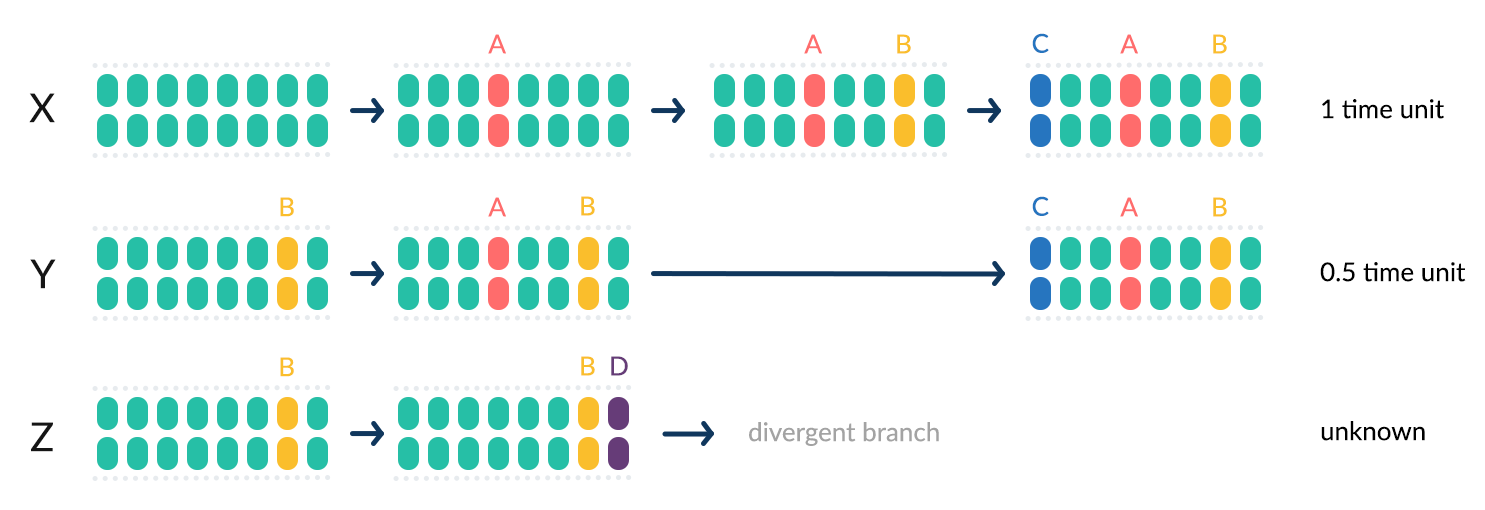
\includegraphics[width=\linewidth]{images/InH.png}
    \caption{Sample hypothesis of inheritance impact on ordered events. (X) shows an assumed regular order A->B->C. This serves as basis of the remaining cases. (Y) and (Z) represent inheritance of the B mutation, which deliver two different outcomes, distinct timing to develop a serious condition and, intrinsically contradicts the established A->B->C order.}
    \label{fig:inh}
\end{figure}

\subsubsection{Hereditary predisposition scenarios}
Put in three simple scenarios where we assume driver mutations which potentially which set off onset of cancer: No Mutation inherited, Heterozygous Mutation inherited and Homozygous Mutation inherited. 
\\

No Mutation reflects the case we have been assuming for gene and pathway alteration event order establishment, in which assortments could be elucidated based purely on observations. Assortment can be then done on what is noticed in the analysis with no external input varying it.
One \emph{advantage} of this scene is that it is commonly expected to have both alleles altered in order to develop a condition (Knudson’s two-hit hypothesis), which implies that if any allele is damaged, at least the other can fill the gap in therms of expression and general contribution to the system. Still, altering the second sister allele can occur at any point.
\\

Heterozygous Mutation implies alteration of only one allele within a gene. This scenario assumes the mutation comes from one of the parents, which increases the probability of acquiring both alleles mutated. This is the so-called \emph{condition predisposition}. In terms of event ordering, this fact shakes the full assortment scheme, as one alteration event can happen regardless of its \emph{"natural" order}, i.e. order inference is broken down due to event displacement. We have observed there can be divergence among the order in which genes/pathways are altered, mainly due to the particular environment each patient has been exposed to. Inheritance is included in the picture too, although in a more disruptive way.
\\

Last, in Homozygous Mutation we assume both alleles have been inherited as mutated. We have observed cases where cancer conditions arise at early ages in some individuals, specially due to this fact. Order discernment is extremely challenging in this case\footnote{We must note, it also depends on the time when the alteration has happened: before or after transmission, which does not exclude the probability of the offspring of developing them naturally.}, since gene mutations would be considered as happening temporarily \emph{early} in progress analysis (Figure \ref{fig:inh} Y). 
In order to tune the discovery, further information coming from first- or second-degree relative shall be illuminating in the quest. This particular case would require a lax model which would allow mutation inheritance, in order to accurately establish a timeline.
\\

Relative importance of gene/pathway order gets now blurred in this scenario. A previously low-ranked event --either due to relevance for not being a serious driver mutation, or because its appearance was expected at a late stage-- might regain interest and be of vital importance if inherited in an altered form. On contrary, it really depends on the effect a mutation has overall, e.g. if its consequences are more related to late stages of the disease (angiogenesis, metastasis, etc.) fatality shall not be reached too soon, although it still supposes a risk.
\\

\subsubsection{Concluding remarks}
All in all, based on the knowledge we have on germline-related study, and also being aware of the lack of a link between gene/pathway chronological order and inheritance significance and impact on its onset, we hypothesise inherited mutations do have an impact on event order in that they clutter the techniques used to accurately establish an assortment. On contrast, somatic alterations are the main \emph{natural} course we'd expect for order decoding, then they can be considered as less detrimental for the order-based approaches.










·······

Since gene-based models are derived to pathway-based, same assumptions are made: If a gene alteration event belongs to early stages of CRC, the pathway it belongs to will too.

········

Pathway "dysregulation speed" is slower than direct gene effect.